\documentclass[11pt]{article}
\usepackage{amsmath, amsfonts, amssymb, graphicx}
\begin{document}
{\textbf{Question 1}}
Method: I first built the function "check" following the iterative formula
provided. I used a loop that gives the next term in the sequence on each
subsequent iteration, checking each iteration if the term's modulus is
greater than 2 since I found a proof detailing that if any term's modulus
is greater than 2, then the sequence diverges. If it does diverge and
if the boolean-valued function "col" is true, then the point will be
assigned a colour dependent on the number of iterations it took for it to
diverge. If col is false, then the point will just be assigned black. If
the point does not diverge within "cap" = 100 iterations of the loop, then
it is assigned the colour white.\\
Following this, I followed some tutorials to learn how to use the
Python imaging library PIL. I found that, essentially, you can
create a blank image of some size and then fill that image in using the
"load" method, iterating over each pixel. So, I iterated over each pixel
and applied a linear function that made each point between -2 and 2, and then
applied my check function, which colours in each pixel. I then outputted
the two plots corresponding to the black and white or rgb plot.\\
\\
Analysis: The two plots are shown below.\\
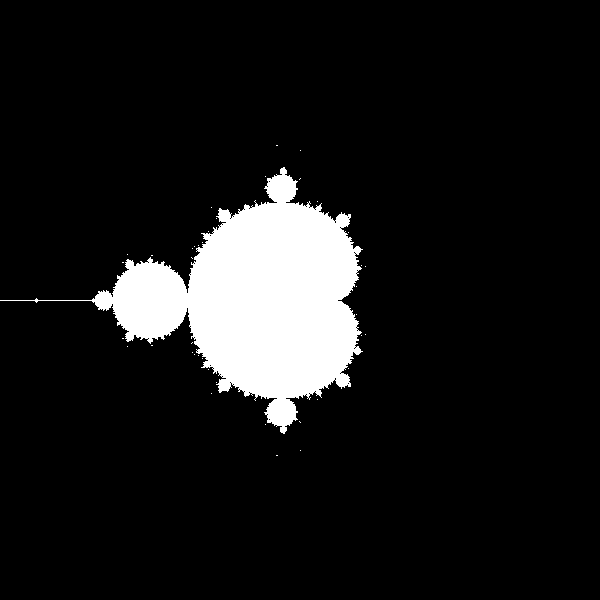
\includegraphics[scale = 0.5]{plot_bw.png}\\
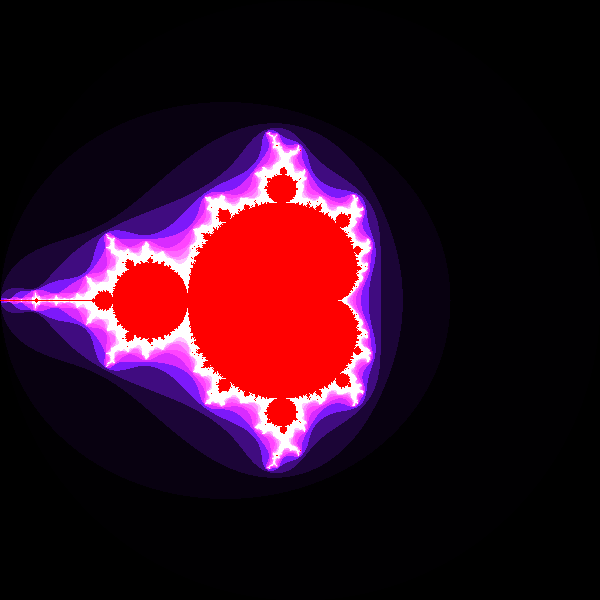
\includegraphics[scale = 0.5]{plot_rgb.png}\\
The plots are a fractal pattern called a mandelbrot set. It is self-similar,
meaning that, zooming in, the pattern observed repeats albeit at a lower scale,
as if the entire set is made up of copies of itself.\\
The right-side lobe is bounded by a shape called a cardioid which is parameterized by a circle rotating around the perimeter of another circle with the same radius. On the rgb plot, brighter colours represent a higher number of iterations
prior to diverging and darker colours a lower number,  and we find that there is like a light to dark gradient
from the boundary out into the rest of the plane. This is intuitive since, as we can see from the black and white plot, the converging points are largely
contained on the interior of the cardioid and secondary lobe, and so the gradient represents the idea that, the further we go away from convergence on the graph, the faster we diverge.\\
\\
{\textbf{Question 2}}\\
Method: I initially created the SIR function, returning the values of the derivatives given the parameters beta and gamma. Then, I looped through the list of parameters, outputting the arrays to plot using scipy numerical integration very similarly to how I learned in class. I used the dop853 algorithm, which is a Runge-Kutta algorithm of order 8 - likely unnecessary but I did so out of curiousity. I found no substantial differences between that and dopri5 (modified RK-4) at the same time-step. I then followed some tutorials to learn how to use the subplots method in matplotlib since I wanted to place all 4 plots on the same plane. I managed to create a grid of plots that is generalizable to however many different different plots (with different parameters) that you please. Though, for odd numbers of plots, it does give an error (still plotting the result) since the empty plot cannot be iterated through. I then repeated this with death added in, following a very similar procedure.\\
\\
Analysis: the plots are shown below\\
\\
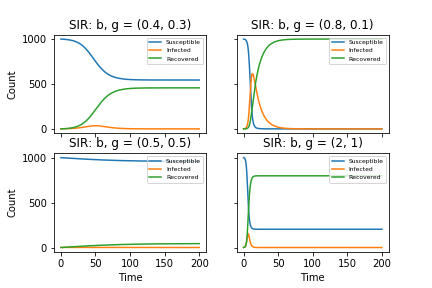
\includegraphics[scale = 0.7]{SIR.png}\\
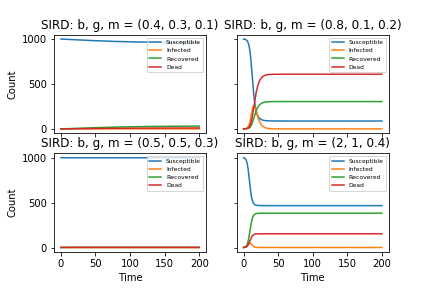
\includegraphics[scale = 0.7]{SIRD.png}\\
The parameters chosen were dependent on the R0 factor, which is defined to be $\frac{\beta*S_0}{\gamma*N}.$ This is defined from the rate of infection, and, if it is greater than 1, then the infection rate rises, leading to an epidemic and possibly pandemic. If it is less than 1, then the infection rate decreases and, if it occurred at the beginning, it means that there will not be a public health crisis. Since $S0 = 999$ and $N = 1000$, $R0$ effectively reduces to $\frac{\beta}{\gamma} < \frac{N}{S0} \approx 1.$\\
In the top left of SIR, we see a situation where there is a public health crisis since the rate of infection ($\beta$) is greater than the rate of recovery ($\gamma$). However, the rates are rather close to one another, and so the "Infected" curve is very flat and small-peaked, indicating that not too many are infected in total, and that it happens over a longer period of time. If deaths are included, then this subdues even faster since the disease cannot spread if the carriers are dead.\\
In the top right of SIR, there is a much more pressing emergency. $\beta >> \gamma,$ and so the number of people infected increases very quickly as indicated by the steep slope of the "Infected" curve and the total number of people infected is large, as indicated by the large area. When death is considered, the situation is not any better since the death rate beats out the recovery rate.\\
In the bottom left of the SIR, there is no pandemic since the infection and recovery rates are equal, not allowing a small number of initially infected individuals to exponentially spread the disease. Adding death does not add anything interesting.\\
Lastly, in the bottom right, larger rates are considered, which, as expected, increase the severity of the slopes of the plots. However, the consequences are not as severe since the recovery rate is objectively high. The death rate is also not as consequential as in the top right.

\end{document}
